\documentclass{book}
\usepackage[paperwidth=36in,paperheight=60in,hmargin=0.75in,vmargin=0.75in]{geometry}
\usepackage{graphicx}
\usepackage{ae}

\begin{document}

\setlength{\unitlength}{1in}
\begin{picture}(34.5,58.5){}
\linethickness{0.125in}

%%%%% POSTER BORDER
\put(0,0.0625){\line(1,0){34.4375}}
\put(0,58.375){\line(1,0){34.4375}}
\put(0,0){\line(0,1){58.4375}}
\put(34.375,0){\line(0,1){58.4375}}

%%%%% TITLE TYPE TEXT
\put(0,55.25){
  \makebox(34.25,2.5){
    \centering
    % title
    \fontsize{180}{200}\selectfont Mapping Chaos
  }
}
\put(0,1.5){
  \makebox(34.25,1.5){
    \centering
    % required siggraph name
    \fontsize{100}{120}\selectfont SIGGRAPH 2004
  }
}
\put(0,0.5){
  \makebox(34.25,1){
    \centering
    % required siggraph location
    \fontsize{80}{100}\selectfont Los Angeles, California
  }
}

\linethickness{0.0625in}
%%%%% IMAGE COMPARISON - HDR TECHNIQUES
%%% text
\put(0.75,14.5){
    \parbox{32.75in}{
    \centering
    \fontsize{60}{70}\selectfont
    Because the image is computed with a high dynamic range, it can be
    interpolated differently to bring out different details. Because
    this step is done separately from computing the image, it can be
    changed in real time, allowing the viewer to tweak the parameters
    to produce the desired effect.
  }
}
%%% base image
\put(0.75,5){
  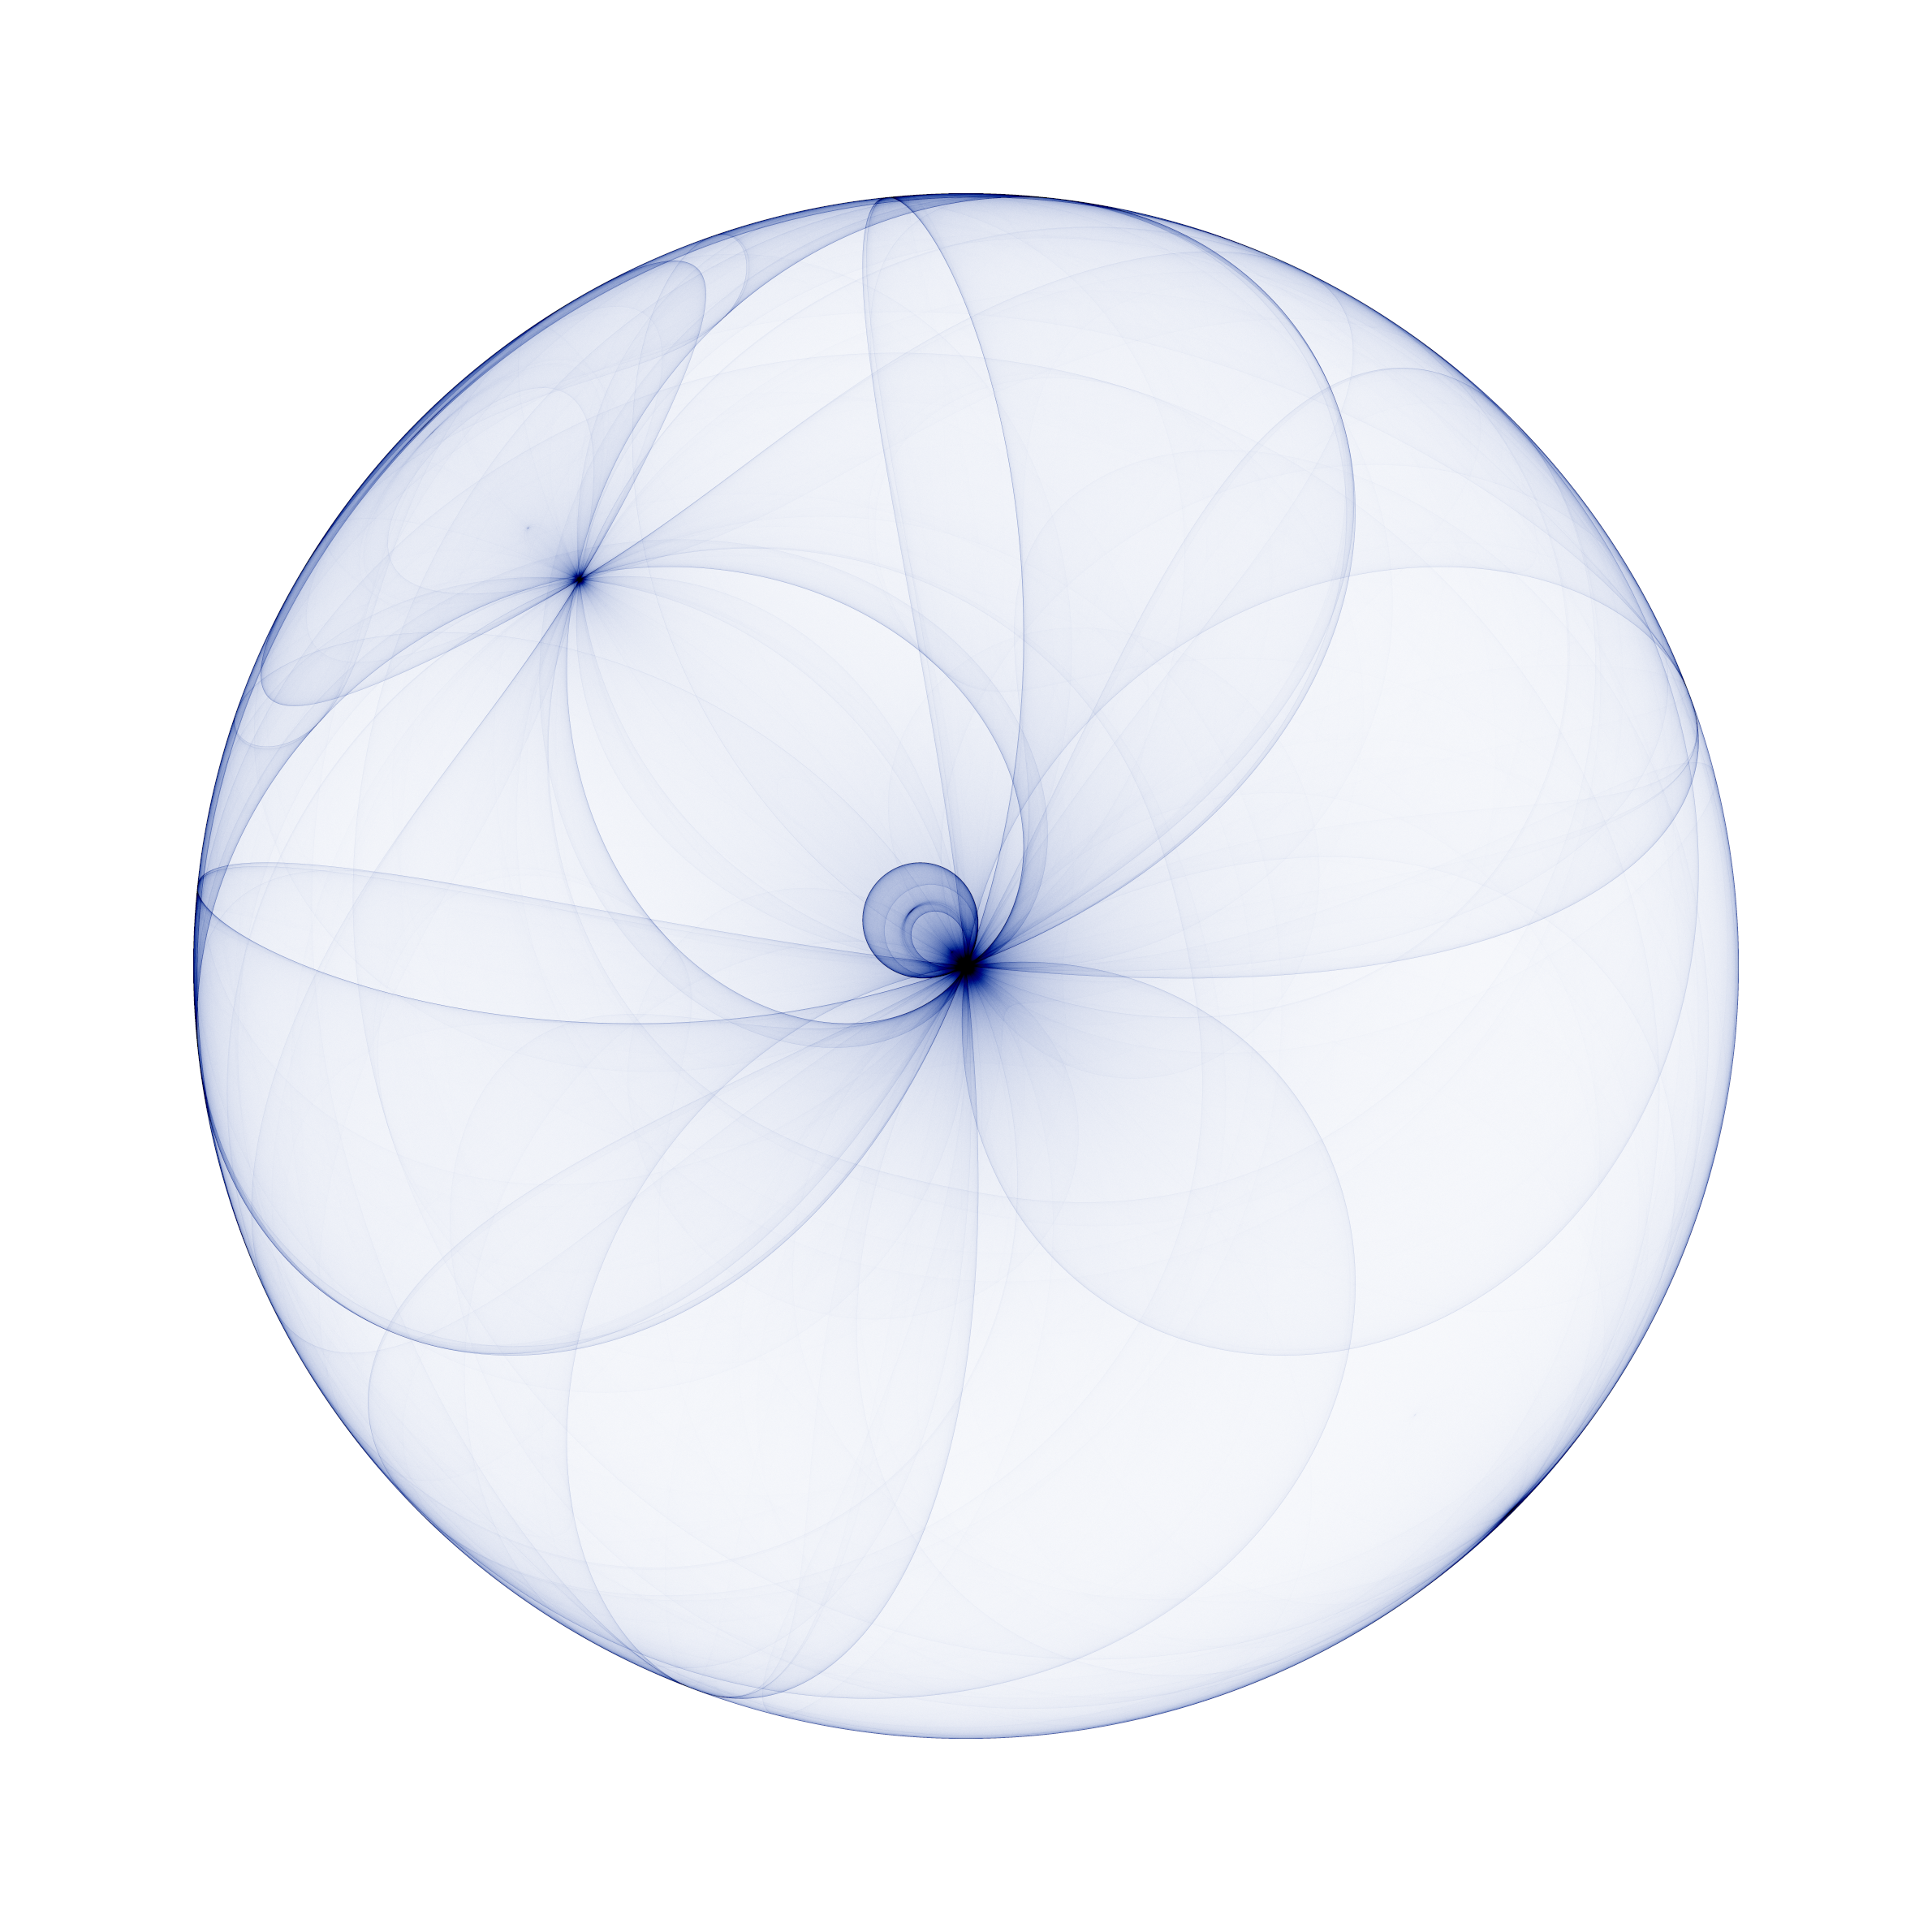
\includegraphics[width=8in]{images/base-large.png}
}
\put(0.75,4){
  \makebox(8,1){
    \centering
    \fontsize{50}{60}\selectfont Base Image
  }
}

%%% increased exposure
\put(8.75,5){
  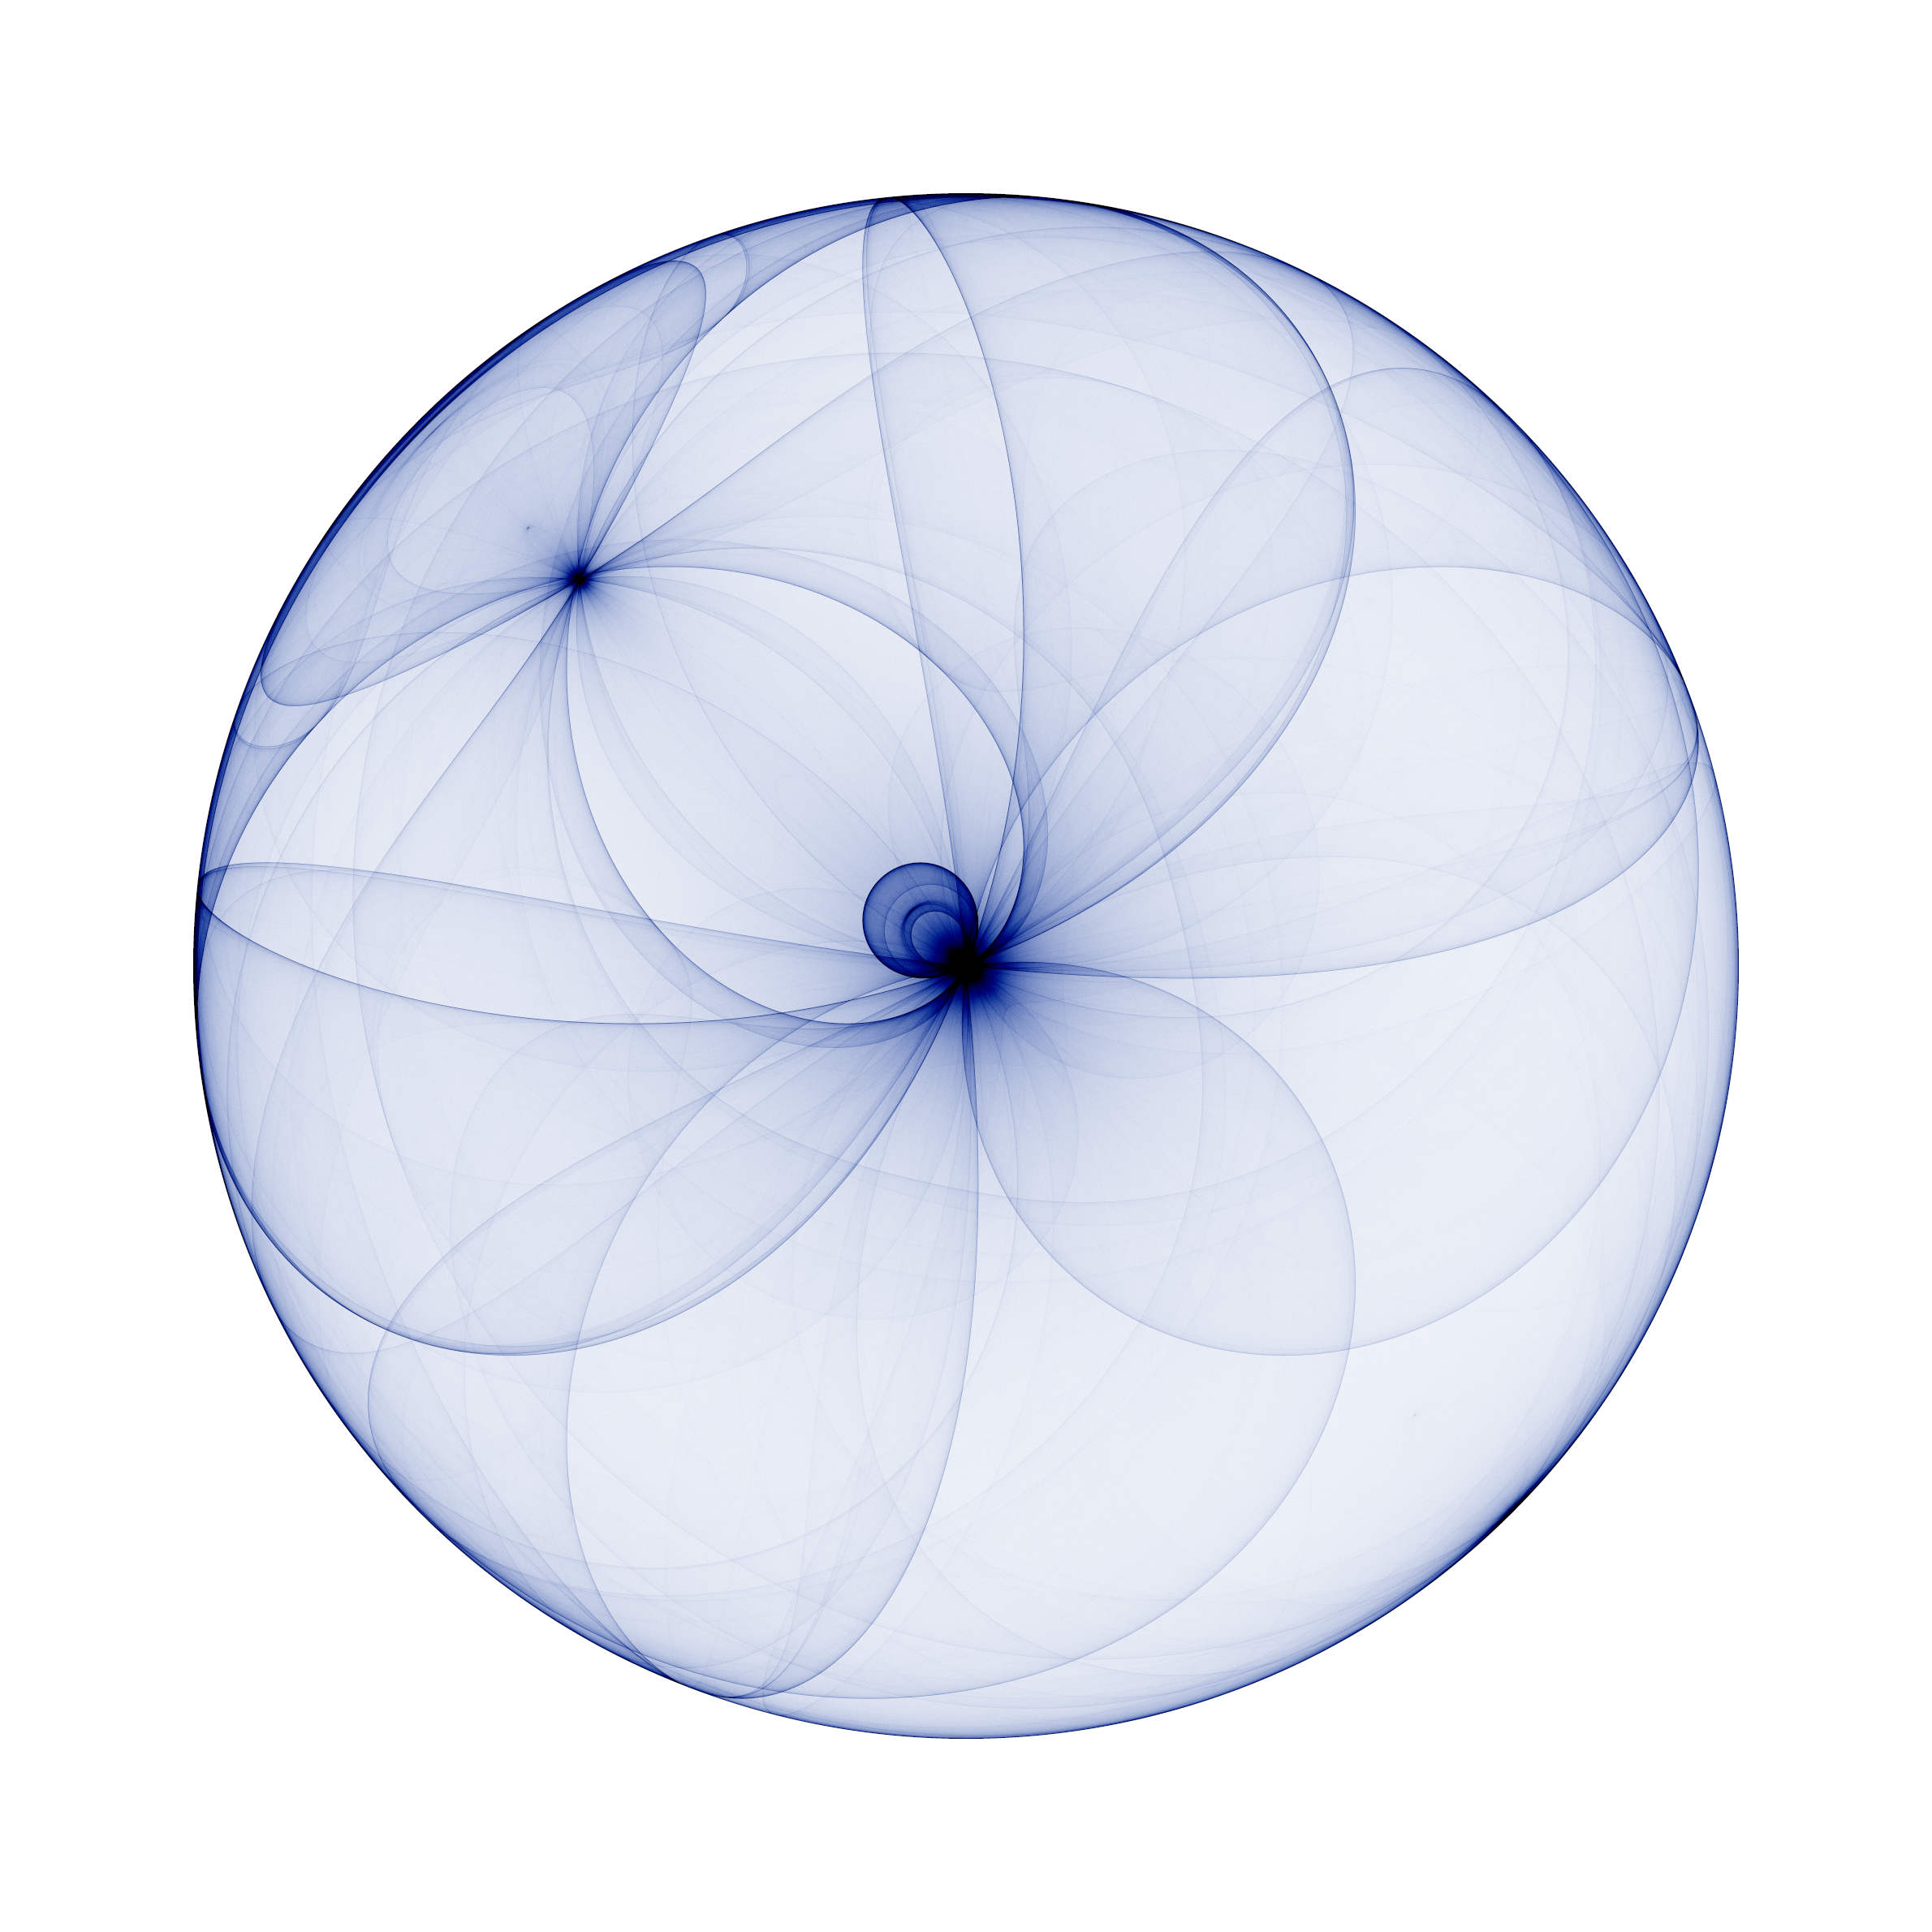
\includegraphics[width=8in]{images/increased-exposure-large.png}
}
\put(8.75,4){
  \makebox(8,1){
    \centering
    \fontsize{50}{60}\selectfont Increased Exposure
  }
}

%%% increased gamma
\put(17.25,5){
  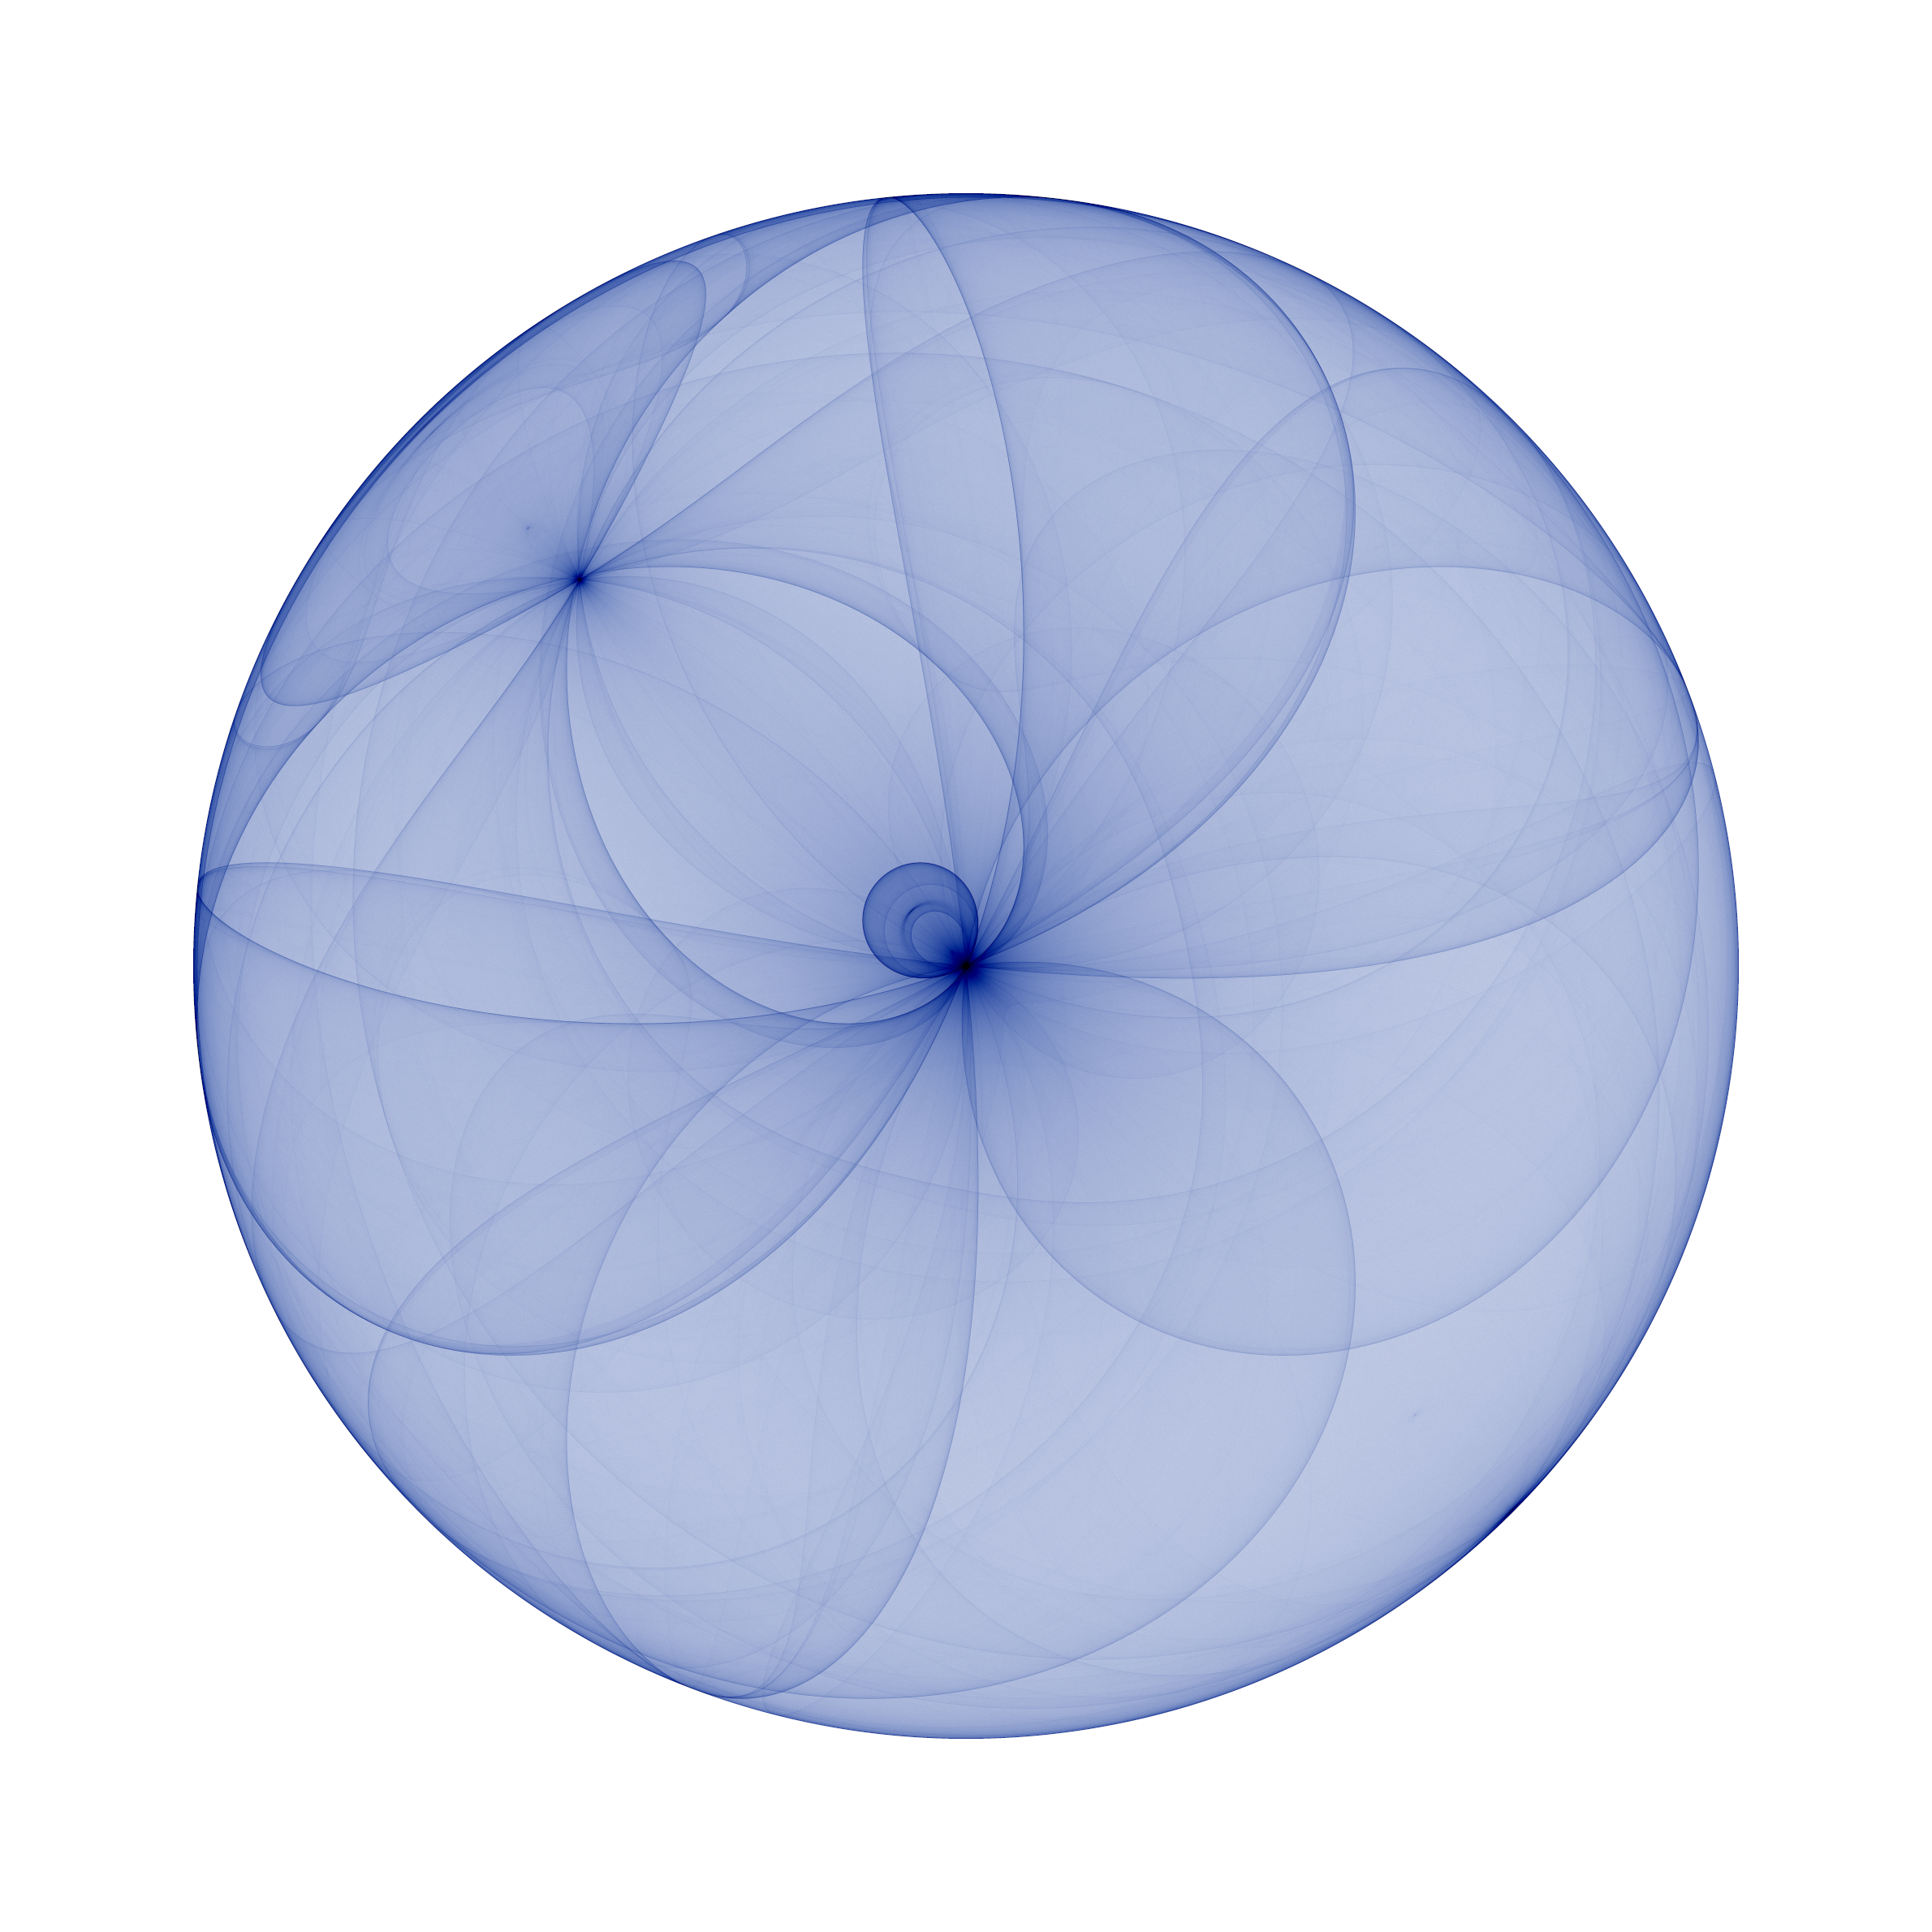
\includegraphics[width=8in]{images/increased-gamma-large.png}
}
\put(17.25,4){
  \makebox(8,1){
    \centering
    \fontsize{50}{60}\selectfont Increased Gamma
  }
}

%%% decreased exposure, increased gamma
\put(25.75,5){
  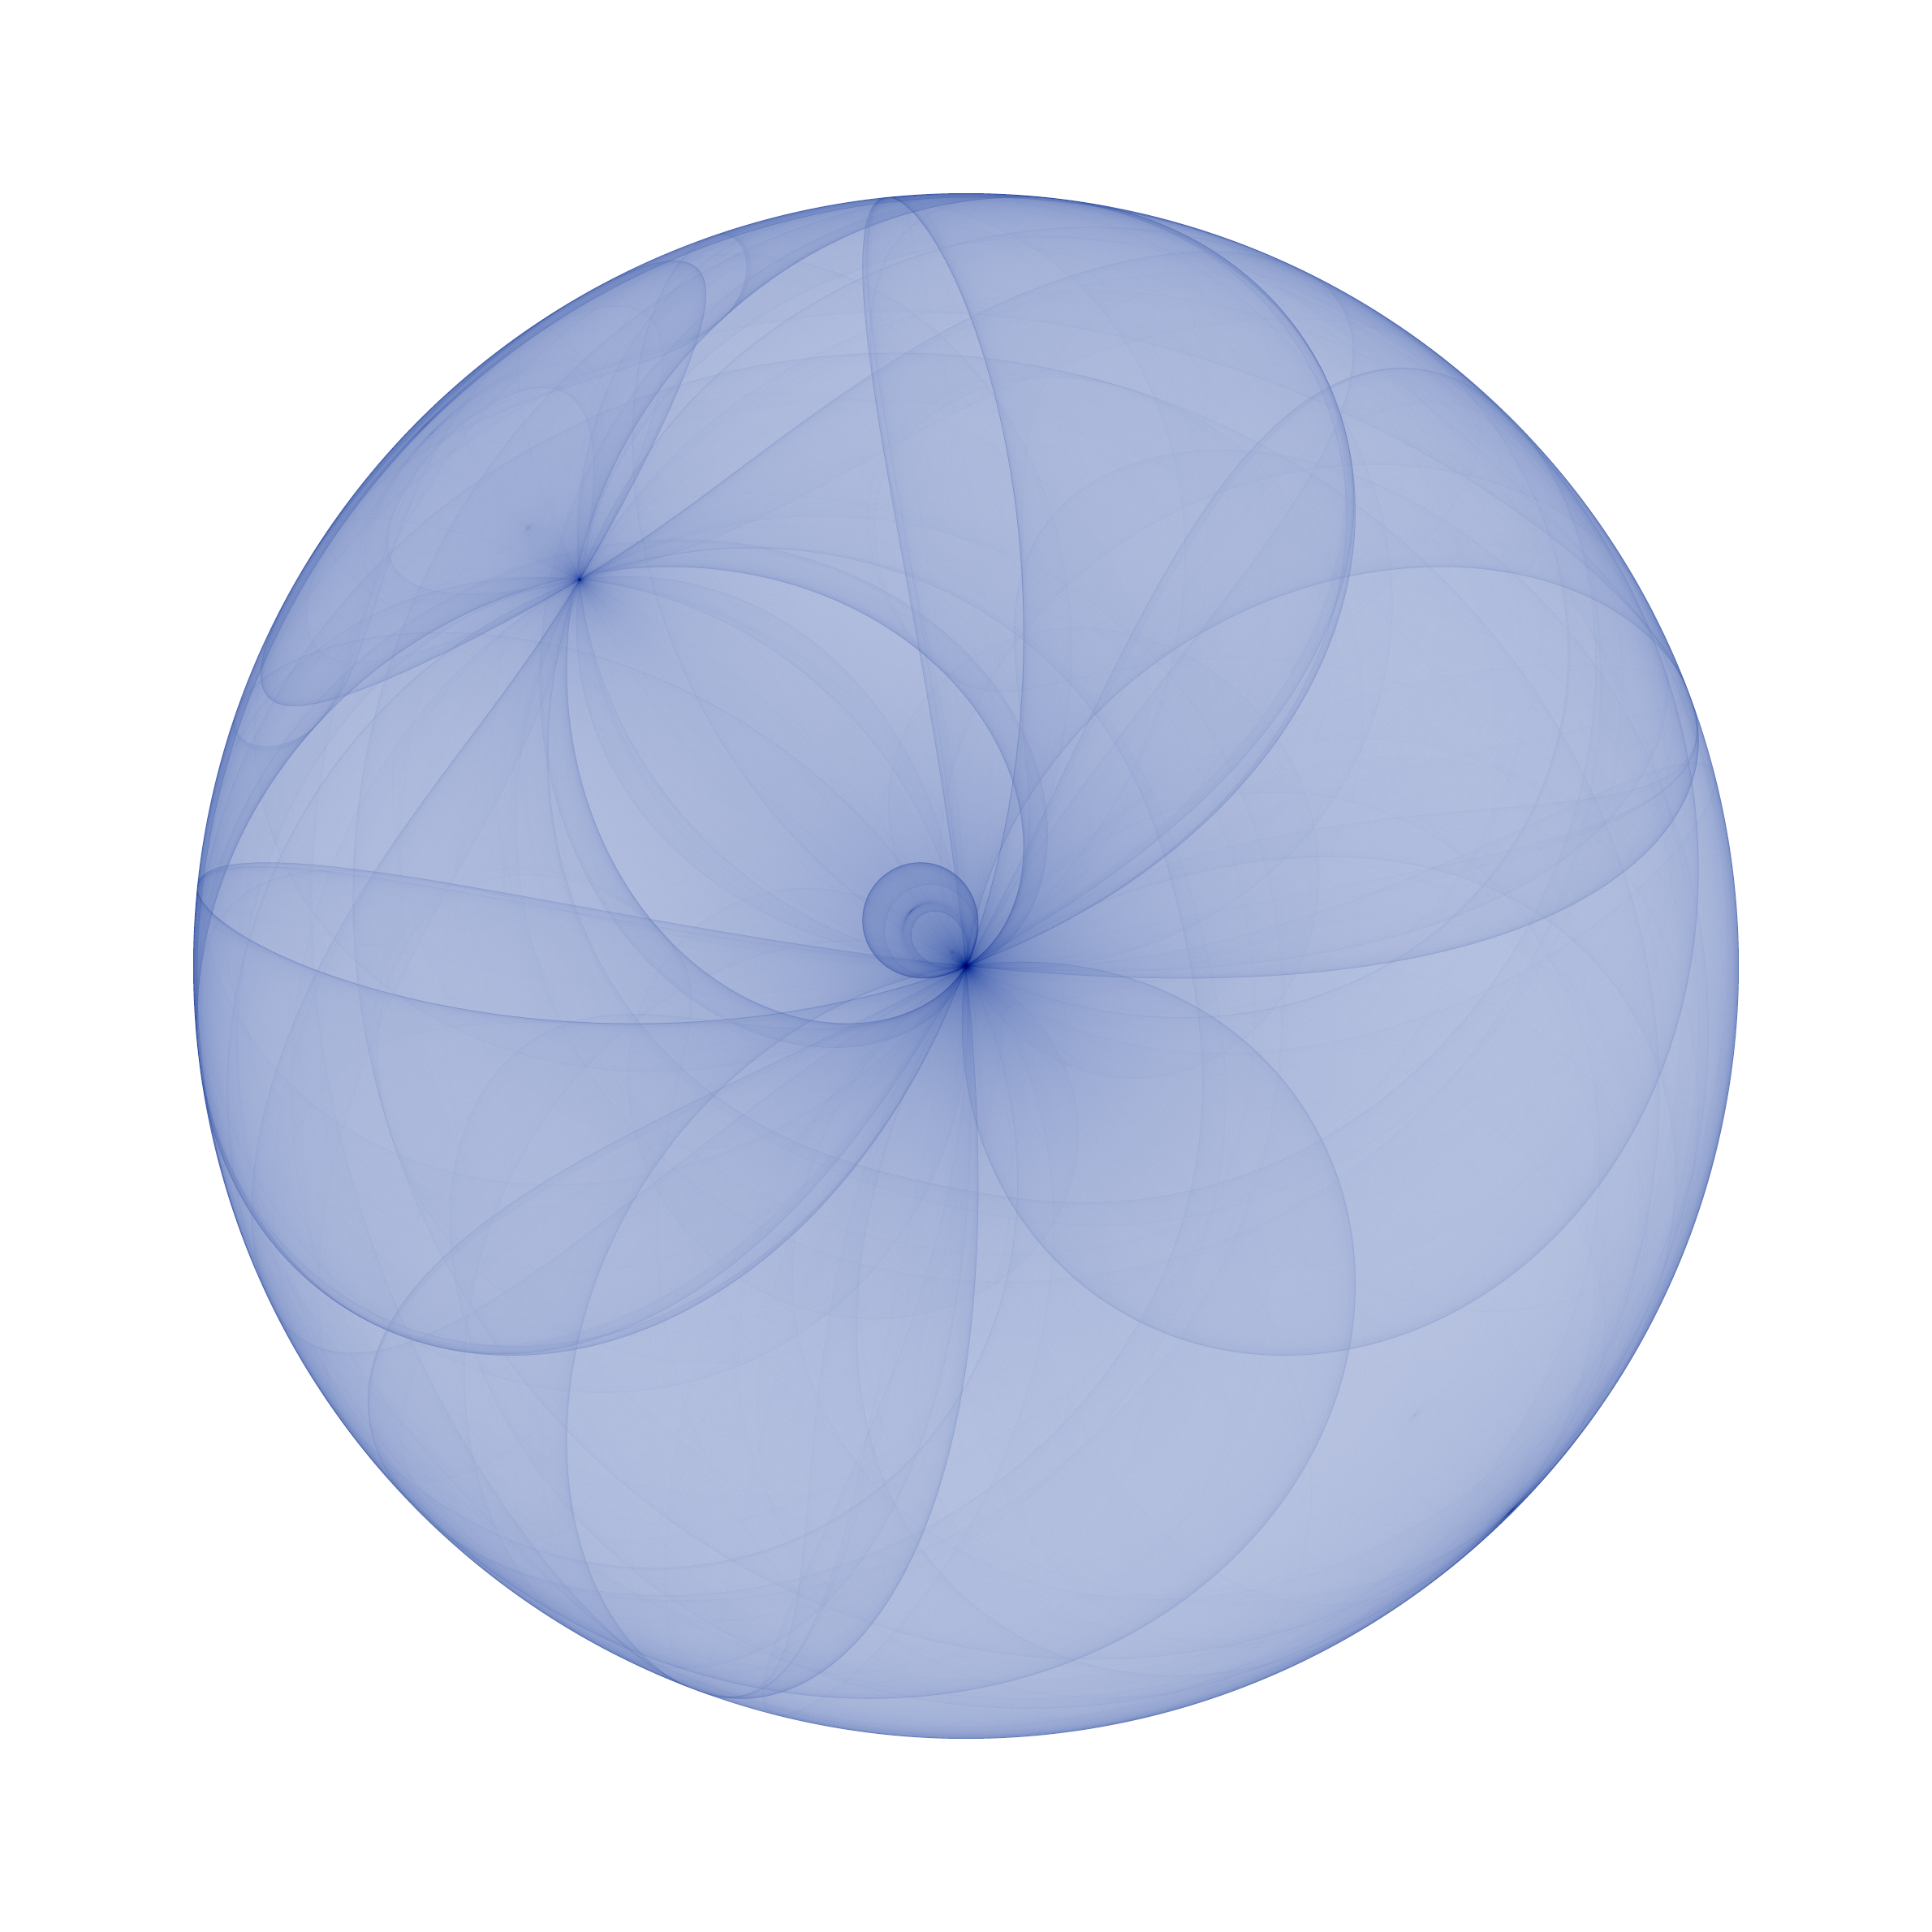
\includegraphics[width=8in]{images/decreased-exposure-increased-gamma-large.png}
}
\put(25.75,4.347){
  \makebox(8,1){
    \centering
    \fontsize{50}{60}\selectfont Decreased Exposure,
  }
}
\put(25.75,3.6527){
  \makebox(8,1){
    \centering
    \fontsize{50}{60}\selectfont Increased Gamma
  }
}

\end{picture}

\end{document}
